\documentclass[12pt]{standalone}

\usepackage{tikz}
\usepackage{ctex}

\begin{document}
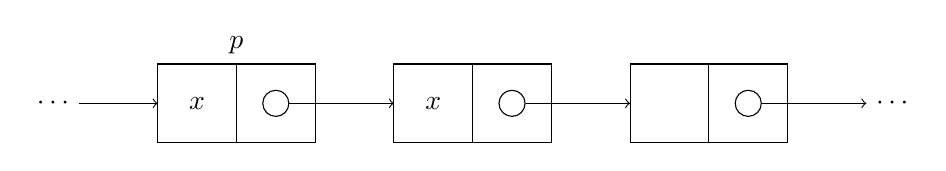
\begin{tikzpicture}

\draw (0,0) rectangle node {$x$} (1,1) 
    (1,0) rectangle node[circle,draw] (A) {} (2,1);
\draw (3,0) rectangle node {$x$} (4,1)
    (4,0) rectangle node[circle,draw] (B) {} (5,1);
\draw (6,0) rectangle node {} (7,1)
    (7,0) rectangle node[circle,draw] (C) {} (8,1);

\draw[->] (-1,0.5) node[left] {$\cdots$} -- (0,0.5);
\draw[->] (A) -- (3,0.5);
\draw[->] (B) -- (6,0.5);
\draw[->] (C) -- (9,0.5) node[right] {$\cdots$};

\node[above] at (1,1) {$p$};

\end{tikzpicture}
\end{document}
